%% RIAI submission format.
%% Elsevier CRC layout used by RIAI: elsarticle (5p) + ecrc_RIAI.sty.
%% Requires the RIAI files in this directory: ecrc_RIAI.sty, elsarticle.cls,
%% elsarticle-harv.bst, RIAIlogo.pdf, SDlogo-5p.pdf, elsevier-logo-5p.pdf.
%% Compile with pdflatex (standard latex will not work).
\documentclass[5p,times,authoryear]{elsarticle}

%% The ecrc package makes the RIAI CRC functionality (running heads, logos) available.
\usepackage{ecrc_RIAI}

\usepackage[utf8]{inputenc}
\usepackage[T1]{fontenc}
\usepackage[spanish,es-noindentfirst]{babel}
\addto\captionsspanish{\def\tablename{Tabla}}
\usepackage{amsmath,amssymb,bm}
\usepackage{graphicx}
\usepackage{booktabs}
\usepackage{url}
\graphicspath{{figs/}}

%% RIAI running-head / logo metadata.
\volume{00}
\firstpage{1}
\journalname{Revista Iberoamericana de Automatica e Informatica industrial}
\jid{RIAI}
\jnltitlelogo{}

%% Authors as they appear in the running head.
\runauth{Scala y López}

\begin{document}

\begin{frontmatter}

\title{Problemas inversos con objetivos mixtos y restricciones de igualdad
sobre redes neuronales sustitutas}

\author[nd]{S. Scala\corref{cor1}}
\ead{simonescala@artelnics.com}
\author[nd]{R. López}
\ead{robertolopez@artelnics.com}
\cortext[cor1]{Autor en correspondencia.}
\address[nd]{Artelnics, Salamanca, España.}

\begin{abstract}
\emph{Copyright {\copyright} 2026 CEA.}\\
El diseño industrial óptimo suele plantearse como la búsqueda de un único punto
óptimo sobre un modelo sustituto entrenado con datos. Muchos problemas de
ingeniería, sin embargo, no piden un óptimo sino \emph{una especificación}: un
valor objetivo que debe alcanzarse exactamente (un acabado, una dureza, una
carga). En este trabajo tratamos el diseño inverso como la recuperación del
\emph{conjunto factible completo} (la variedad de soluciones) que satisface una
especificación impuesta como restricción de igualdad sobre la salida de una red
neuronal sustituta. Sobre ese planteamiento construimos un esquema de
optimización de respuesta de \emph{sentido mixto}, en el que distintas salidas
del mismo problema pueden minimizarse, maximizarse o fijarse simultáneamente, y
un criterio de selección que ordena las soluciones de la variedad por su
\emph{robustez}, calculada con el Jacobiano analítico de la red, equilibrada con
su centralidad en el dominio. El método maneja de forma nativa restricciones de
caja, afines (incluido el símplex composicional) y no lineales. Lo validamos en
dos casos con datos reales y solo variables numéricas: el torneado CNC de acero
de herramienta AISI H13 (fijar la rugosidad y recorrer el compromiso entre fuerza de corte y
tasa de arranque de material) y la dureza de aleaciones de alta
entropía sobre el símplex de composición (fijar la dureza y recuperar la
variedad de aleaciones factibles). En ambos casos se recupera una variedad rica
y diversa de diseños que cumplen la especificación, con satisfacción exacta de
las restricciones afines, y se selecciona de ella el diseño más robusto. Una
comparación honesta, en la que damos la misma reparación a las líneas base,
muestra que la reparación es el factor decisivo de factibilidad (sin ella la
restricción de símplex es inviable por muestreo) y que la aportación propia del
método son los objetivos de sentido mixto y la selección por robustez; con el mismo
presupuesto de evaluaciones, nuestro método iguala a los mejores optimizadores de
propósito general en el objetivo escalar y además devuelve, en la misma pasada, la
variedad completa y su ordenación por robustez. En el caso de dominio de caja, la
variedad que recupera es además la que menos extrapola el sustituto: se mantiene más
cerca de los datos de entrenamiento que las de las líneas base.
\end{abstract}

\begin{keyword}
diseño inverso \sep optimización de respuesta \sep redes neuronales sustitutas
\sep restricciones de igualdad \sep robustez \sep objetivos mixtos
\end{keyword}

\end{frontmatter}

\section{Introducción}
\label{sec:intro}

La cadena habitual del diseño industrial guiado por datos entrena un modelo
sustituto $f:\mathbb{R}^p\to\mathbb{R}^q$ (a menudo una red neuronal) sobre
medidas experimentales o de simulación, y después busca condiciones de operación
que optimicen una o varias salidas. En un trabajo companion abordamos esta búsqueda
como \emph{optimización de respuesta}, con estrategias sin derivadas que explotan el
bajo coste de evaluar la red y proyectan (reparan) las muestras sobre las
restricciones antes de evaluarlas, garantizando la factibilidad por construcción
\citep{scala2026idc}. El operador de reparación de restricciones es maquinaria común
de esa línea; en este trabajo lo reutilizamos y no lo reclamamos como aportación.

Aquel planteamiento devuelve un único óptimo factible (o un frente de Pareto). Aquí
adoptamos una perspectiva distinta, la del \emph{problema inverso}. Además, una
parte importante de los problemas de ingeniería no se formula como
``optimizar'', sino como ``alcanzar una especificación'': fabricar una pieza con
un acabado superficial dado, una aleación con una dureza dada, un proceso que
opere a una carga dada. En estos casos el objetivo natural es una
\emph{restricción de igualdad} sobre la salida, $f_k(\mathbf{x})=c$, y su
solución no es un punto sino una \emph{variedad}: el conjunto de todas las
recetas que cumplen la especificación. Recuperar esa variedad, en lugar de un
solo representante, tiene valor práctico directo: permite elegir después, entre
todas las soluciones equivalentes en la especificación, la que mejor satisface
criterios secundarios (coste, productividad) o la más robusta frente a errores
de fabricación.

Este artículo desarrolla esa idea con tres contribuciones. Primera, planteamos
el diseño inverso como la recuperación de la variedad factible definida por una
o varias restricciones de igualdad sobre la red sustituta
(Sección~\ref{sec:metodo}). Segunda, generalizamos la formulación a
\emph{objetivos de sentido mixto}, en los que sobre un mismo problema conviven
salidas a minimizar, a maximizar y a fijar. Tercera, introducimos un criterio de
selección que ordena las soluciones de la variedad por robustez, medida con el
Jacobiano analítico de la red y ponderada por el dominio, y la equilibra con la
centralidad del punto en la caja de diseño. Al tratarse de una recuperación de
conjunto y no de una relajación, la especificación puede exigirse además de forma
\emph{exacta}, sin tolerancia elegida por el usuario, algo que el muestreo por rechazo
no alcanza. El método se valida en dos casos con
datos reales y variables numéricas (Secciones~\ref{sec:cnc} y~\ref{sec:hea}).

\section{Optimización de respuesta de sentido mixto}
\label{sec:metodo}

\subsection{Planteamiento}
Sea $f:\mathcal{X}\subseteq\mathbb{R}^p\to\mathbb{R}^q$ una red neuronal
entrenada, con entradas $\mathbf{x}$ acotadas a una caja
$\mathcal{X}=\prod_i[l_i,u_i]$. A cada salida $j$ se le asigna un \emph{sentido}
$s_j\in\{\text{min},\text{max},\text{fijo}\}$. Las salidas ``fijo'' llevan un
valor objetivo $c_j$; las salidas ``min''/``max'' definen los objetivos de
optimización. Además se admiten restricciones sobre entradas y salidas: de caja,
afines $\mathbf{a}^\top\mathbf{x}\bowtie\beta$ (incluido el símplex
$\sum_i x_i = 1$) y no lineales $g(\mathbf{x})\bowtie\beta$.

\subsection{Objetivo fijo y variedad factible}
Un objetivo de igualdad $f_k(\mathbf{x})=c_k$ se impone como una banda estrecha
$|f_k(\mathbf{x})-c_k|\le\varepsilon$ alrededor del valor objetivo. El
optimizador muestrea el dominio, repara las muestras sobre las restricciones
afines, evalúa la red y retiene las que caen en la banda, contrayendo
iterativamente el dominio alrededor de la región factible. El resultado no es un
punto sino un conjunto de soluciones $\{\mathbf{x}^{(r)}\}$ que aproxima la
variedad $\mathcal{M}_c=\{\mathbf{x}\in\mathcal{X}: f_k(\mathbf{x})=c_k\}$.

La banda $\varepsilon$ es solo un \emph{mecanismo de recolección}: sirve para
retener muchos puntos de la variedad, no para relajar la especificación. Como la
contracción del dominio concentra el muestreo alrededor del valor objetivo, el
método no necesita que el usuario fije una tolerancia; puede pedirse el valor
\emph{exacto} ($\varepsilon\to0$) y la contracción sigue devolviendo un conjunto
poblado de soluciones cuyo residuo $|f_k(\mathbf{x})-c_k|$ tiende a cero. Esto
distingue el planteamiento del muestreo por rechazo, que no puede acertar un
objetivo de medida nula: su conjunto factible se vacía al estrechar la banda
(Sección~\ref{sec:baselines}).

\subsection{Sentidos mixtos}
Cuando junto a una salida fija coexisten salidas a minimizar o maximizar, la
igualdad se mantiene como banda y los sentidos min/max se optimizan sobre ella,
devolviendo el frente de compromiso restringido a la variedad. Así, un mismo
problema puede, por ejemplo, \emph{fijar} una salida y \emph{minimizar} otra, como en el
Caso~A (Sección~\ref{sec:cnc}: fijar $R_a$, minimizar $F$), donde además la tasa de
arranque de material (MRR) --función analítica de las entradas-- se recorre como
compromiso a lo largo de la variedad. Fijar simultáneamente dos salidas
($f_{k_1}=c_1$ y $f_{k_2}=c_2$) recupera la intersección de dos variedades.

\subsection{Robustez y selección}
\label{sec:robustez}
Todas las soluciones de $\mathcal{M}_c$ cumplen la especificación por igual; se
distinguen por su sensibilidad a errores en las entradas. Definimos la robustez
de una solución mediante el Jacobiano analítico de la red, ponderado por el
tamaño del dominio de cada entrada,
\begin{equation}
S(\mathbf{x}) \;=\;
\sqrt{\sum_{i=1}^{p}\Big(\frac{\partial f_k}{\partial x_i}(\mathbf{x})\,
(u_i-l_i)\Big)^{2}} ,
\label{eq:sens}
\end{equation}
de modo que $S$ estima la deriva de la salida si cada entrada se desviara en una
fracción de su rango. Un valor menor indica un diseño más manufacturable. El
Jacobiano se obtiene con el mismo motor de diferenciación que emplea el
optimizador (validado frente a diferencias finitas). Para combinarla con la
centralidad, normalizamos $S$ al intervalo $[0,1]$ sobre el conjunto devuelto y la
invertimos, $R(\mathbf{x})=1-\hat S(\mathbf{x})$ (mayor $R$, más robusto). La
selección final combina esa robustez $R$ y la \emph{centralidad} $C(\mathbf{x})$,
definida como el menor margen normalizado de la solución a las paredes de la caja de
diseño ($1$ en el centro, $0$ sobre una pared), con un único parámetro
$\alpha\in[0,1]$ mediante la media geométrica $C^{1-\alpha}\,R^{\alpha}$, de forma
que $\alpha=0$ elige el diseño más central y $\alpha=1$ el más robusto.

La centralidad no es un mero desempate: es una salvaguarda frente al propio modelo.
La robustez $S$ se estima con el Jacobiano del \emph{sustituto}, y ese sustituto
solo es fiable dentro del soporte de los datos de entrenamiento. Una solución con
margen pequeño se sitúa en el borde de la caja, justo donde la red extrapola y sus
unidades se saturan; allí su Jacobiano, y por tanto la robustez que le atribuimos,
es menos digno de confianza. Por eso, ante el riesgo de extrapolación, conviene
preferir un punto más central (un $\alpha$ moderado, en torno a $0.5$) que sacrifica
algo de robustez nominal a cambio de una predicción en la que podemos confiar. La
selección se resuelve sobre cada variedad por separado, de modo que el punto
equilibrado depende de la geometría concreta de $\mathcal{M}_c$.

\section{Caso A: torneado CNC de AISI H13}
\label{sec:cnc}

\paragraph{Datos y sustituto} Partimos de una campaña factorial replicada de
torneado de acero de herramienta AISI H13 \citep{canal2022}. Las
variables de decisión (numéricas) son la velocidad de corte $v_c$, el avance $f$
y la profundidad de pasada $a_p$, junto con el estado de desgaste de la
herramienta $VB$ tratado como variable numérica. Las respuestas son la rugosidad
media $R_a$ y la fuerza de corte resultante $F$; la tasa de arranque de material
$\mathrm{MRR}=v_c\,f\,a_p$ es analítica. Entrenamos una red sustituta
multisalida $(v_c,f,a_p,VB)\to(R_a,F)$ con selección de arquitectura de neuronas.
La fuerza se predice con precisión ($R^2\approx0.99$); la rugosidad, dominada por
el avance pero con dispersión de réplicas, alcanza $R^2\approx0.7$ y su
dispersión define la tolerancia natural de la banda de igualdad.

\paragraph{Diseño de sentido mixto} Planteamos el problema mixto: \emph{fijar}
$R_a$ en una especificación de acabado y recuperar la variedad de recetas que la
cumplen, sobre la cual la fuerza $F$ (a minimizar) y la productividad $\mathrm{MRR}$
(a maximizar) se contraponen. Fijado el objetivo de rugosidad en un valor alcanzable del
rango del sustituto (aquí $R_a\approx0.62~\mu$m), el optimizador recupera una variedad de
\textbf{3400 recetas} que mantienen $R_a$ dentro de la banda
$[0.605,0.638]~\mu$m. Sobre esa variedad, la fuerza recorre
$[95,402]$~N y la MRR $[8.0,27.5]$, de modo que ambos criterios compiten a lo largo del
conjunto factible y uno elige la receta según su prioridad
(Figura~\ref{fig:cnc_tradeoff}). Como el problema solo tiene tres palancas
continuas, la variedad de $R_a$ constante es una superficie bidimensional
directamente visualizable en el espacio de decisión
(Figura~\ref{fig:cnc_3d}).

\begin{figure}[t]
\centering
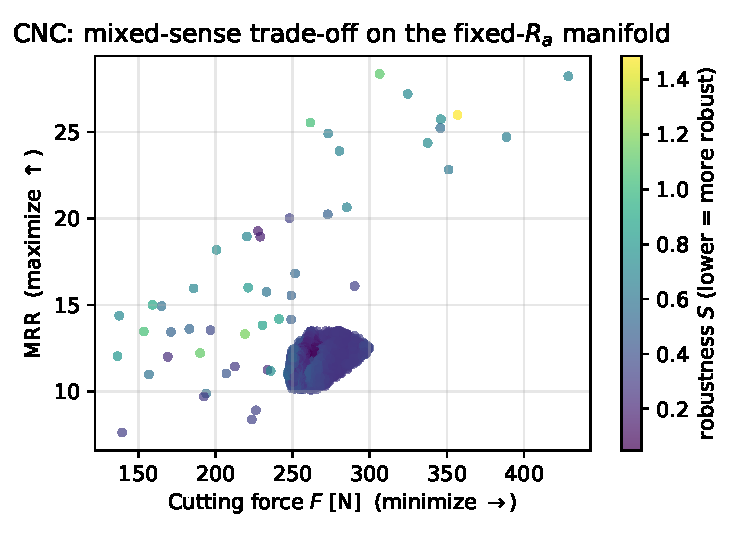
\includegraphics[width=\linewidth]{fig_cnc_tradeoff.pdf}
\caption{Caso A. Compromiso de sentido mixto sobre la variedad de $R_a$ fijo:
cada punto es una receta con la rugosidad en la especificación; el eje horizontal
es la fuerza a minimizar y el vertical la MRR a maximizar, coloreados por la
robustez $S$ de la ecuación~\eqref{eq:sens}.}
\label{fig:cnc_tradeoff}
\end{figure}

\begin{figure}[t]
\centering
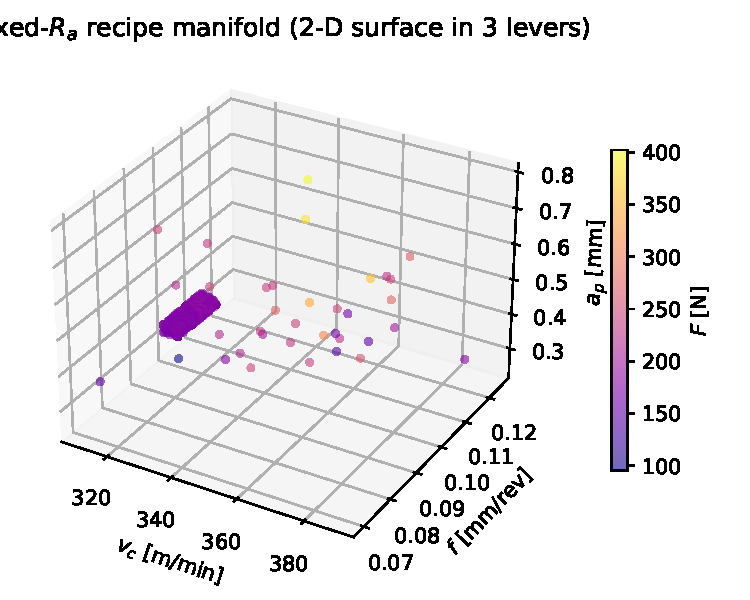
\includegraphics[width=\linewidth]{fig_cnc_manifold3d.pdf}
\caption{Caso A. La variedad de recetas con $R_a$ fijo es una superficie
bidimensional en las tres palancas continuas $(v_c,f,a_p)$, coloreada por la
fuerza de corte $F$.}
\label{fig:cnc_3d}
\end{figure}

\paragraph{Selección y multiobjetivo de igualdad} El criterio de la
Sección~\ref{sec:robustez} devuelve recetas distintas según $\alpha$ (más central
frente a más robusta), que difieren claramente en fuerza y productividad sobre la
misma especificación de rugosidad. La diferencia no es solo de valor: sobre esta
variedad de 3400 recetas, la receta de robustez pura ($\alpha=1$) tiene un margen a
las paredes de apenas $0.04$, es decir, se apoya casi sobre el borde de la caja de
entrenamiento, donde el sustituto extrapola; al bajar a $\alpha=0.5$ y $\alpha=0$ el
margen sube a $0.51$ y $0.58$, devolviendo recetas en el interior bien muestreado del
dominio. En la práctica preferimos ese punto más central como cobertura frente al
riesgo de extrapolación del modelo (Sección~\ref{sec:robustez}). Al añadir la
minimización explícita de $F$ bajo la rugosidad fija, el solver alcanza una receta de
fuerza mínima ($F\approx78$~N). Finalmente, fijando
simultáneamente $R_a$ y $F$ se recupera la intersección de ambas variedades
(5100 soluciones), que ilustra la capacidad multiobjetivo de igualdad.

\section{Caso B: dureza de aleaciones de alta entropía sobre el símplex}
\label{sec:hea}

\paragraph{Datos y sustituto} El segundo caso usa una tabla pública de dureza
Vickers de aleaciones de alta entropía \citep{yang2022}. Las entradas son las diez
fracciones atómicas (Al, Co, Cr, Cu, Fe, Mn, Mo, Ni, Ti, V), que suman uno, y la
salida es la dureza $HV$. El sustituto alcanza $R^2\approx0.87$ sobre 370
aleaciones. La composición impone la restricción afín de \emph{símplex}
$\sum_i x_i = 1$, la prueba canónica del operador de reparación afín.

\paragraph{Recuperación de la variedad de aleaciones} Fijamos la dureza en un
valor alcanzable ($HV\approx538$) y recuperamos la variedad de composiciones que
la producen. El optimizador devuelve \textbf{183 aleaciones} distintas, todas
sobre el símplex con error máximo $|\sum_i x_i-1|=0$ (satisfacción exacta de la
restricción afín). La variedad es diversa: cada fracción recorre entre el 39\% y
el 99\% de su rango admisible (Figura~\ref{fig:hea_parallel}), lo que muestra que
existen familias de aleaciones muy distintas con la misma dureza. Sobre ese
conjunto, la robustez de la ecuación~\eqref{eq:sens} separa las composiciones
poco sensibles a la variación de composición de las muy sensibles, y la selección
centralidad--robustez recomienda la aleación más manufacturable.

\begin{figure*}[t]
\centering
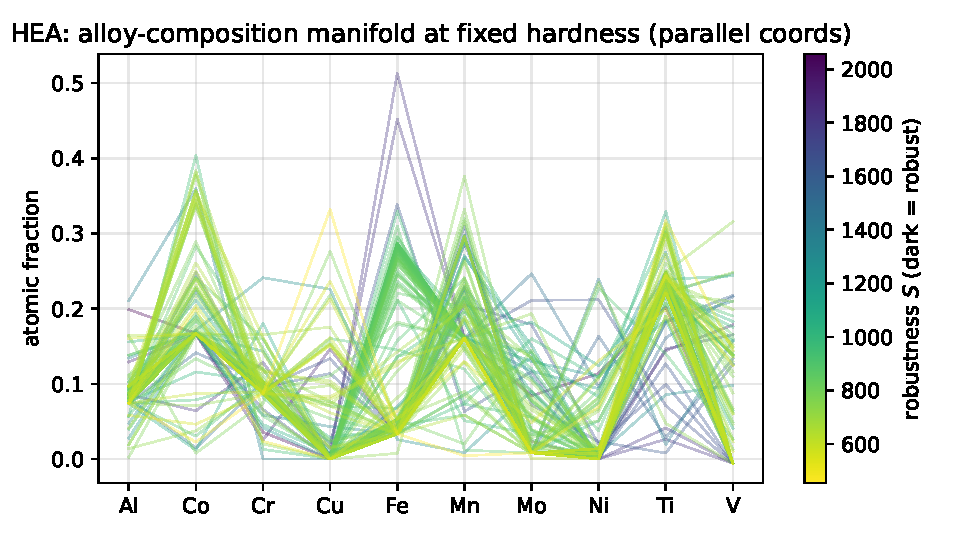
\includegraphics[width=0.9\linewidth]{fig_hea_parallel.pdf}
\caption{Caso B. Variedad de composiciones con dureza fija, en coordenadas
paralelas sobre las diez fracciones atómicas (suma uno). El color codifica la
robustez $S$; las trayectorias oscuras son las aleaciones más robustas.}
\label{fig:hea_parallel}
\end{figure*}

\section{Comparación honesta con líneas base}
\label{sec:baselines}
Para separar la aportación real del método de la de la reparación, damos a las
líneas base \emph{el mismo operador de reparación} que usa nuestro método. Sobre
un presupuesto comparable de evaluaciones y con un criterio de factibilidad
idéntico (banda de igualdad en la salida más la restricción de símplex en las
entradas), comparamos: muestreo por rechazo \emph{sin} reparación; muestreo por
rechazo \emph{con} reparación (una ronda de muestreo, reparación afín de entradas,
reparación de la salida y filtrado, exactamente los mismos operadores); nuestro
método iterativo con contracción del dominio; y, para el objetivo escalar, las
metaheurísticas de propósito general de \texttt{pymoo} \citep{blank2020pymoo}. Todas las líneas base reciben el
mismo sustituto congelado, las mismas restricciones y el mismo presupuesto de
evaluaciones. La Tabla~\ref{tab:base} resume los resultados y la Figura~\ref{fig:extrap}
ilustra el análisis de extrapolación que los distingue.

\begin{figure*}[t]
\centering
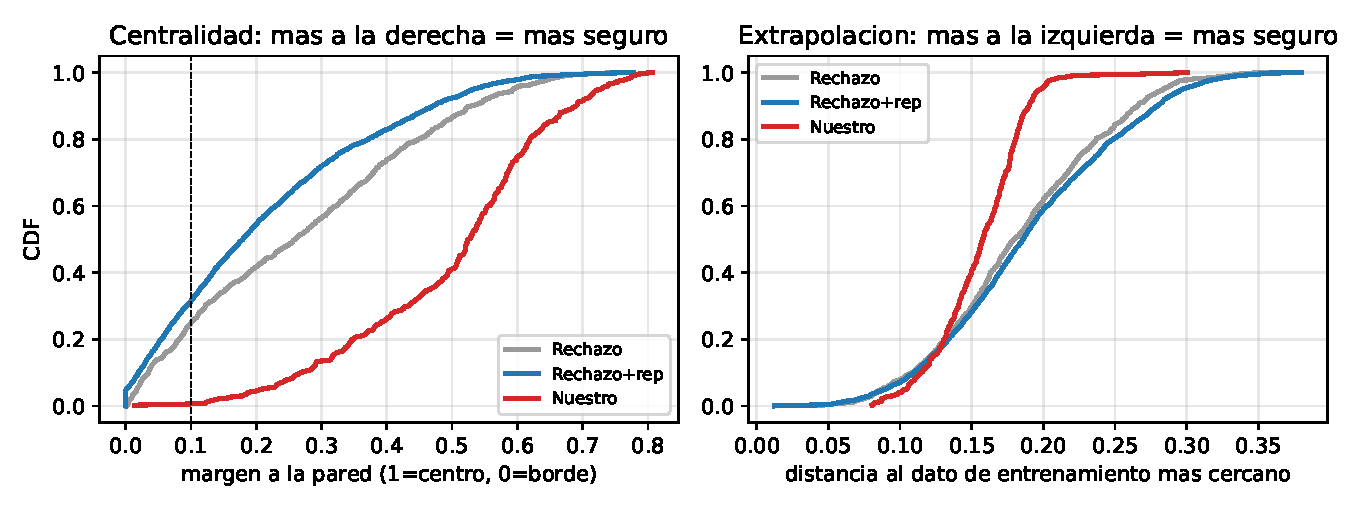
\includegraphics[width=0.9\linewidth]{fig_extrapolation_cnc.pdf}
\caption{Distribución (CDF) sobre \emph{toda} la variedad factible de la CNC. Izquierda:
centralidad (margen a la pared); más a la derecha es más seguro. Derecha: distancia al
dato de entrenamiento más cercano; más a la izquierda es más seguro. Nuestra variedad
(rojo) es favorable en ambos paneles: se mantiene en el interior del dominio y cerca de los
datos; el rechazo (gris/azul) se dispersa hacia el borde y se aleja más del dato.}
\label{fig:extrap}
\end{figure*}

\paragraph{Protocolo} El presupuesto es de $1.2\times10^4$ evaluaciones del sustituto
para todos los métodos, contado con el número real de propagaciones directas (incluidas
las de la reparación). Para que la comparación sea estrictamente equitativa, ajustamos
nuestro método a $6$ iteraciones de $2\times10^3$ muestras: con esta configuración la
contracción no puede detenerse antes de la última iteración, de modo que \emph{gasta el
presupuesto completo} y usa exactamente las mismas $1.2\times10^4$ evaluaciones que el
resto (evitamos así cualquier ventaja aparente por terminar antes). Las metaheurísticas de
\texttt{pymoo} (GA, DE, PSO con población $100$; CMA-ES con reinicios IPOP) usan una
terminación por número de
evaluaciones para igualar exactamente el presupuesto. Todas reciben el mismo sustituto
congelado, las mismas restricciones y el mismo operador de reparación; el criterio de
factibilidad (banda de igualdad más símplex) es idéntico.

\begin{table}[t]
\centering
\caption{Comparación con la misma reparación, mismo presupuesto de evaluaciones
($1.2\times10^4$ para todos los métodos) y criterio de factibilidad idéntico (banda de
igualdad y símplex). Cobertura = relleno medio del dominio por las soluciones factibles;
robustez = menor $S$ disponible en el conjunto devuelto (selección posterior, menor es
mejor; ningún método optimiza $S$). Caso CNC; la HEA se comenta en el texto.}
\label{tab:base}
\begin{tabular}{lcccc}
\toprule
Método & Reparación & Factib. & Cobertura & Robustez mín $S$ \\
\midrule
Rechazo          & no & 7.5\%  & 99.6\%  & 0.092 \\
Rechazo          & sí & \textbf{21.5\%} & \textbf{99.9\%} & \textbf{0.067} \\
Nuestro (iterativo) & sí & 3.1\%  & 72.3\%  & 0.108 \\
\bottomrule
\end{tabular}
\end{table}

De aquí extraemos conclusiones \emph{honestas}, y ninguna consiste en que un método
domine a los demás. Primera, la reparación es el factor decisivo de factibilidad:
sin ella la restricción de símplex de la HEA es inviable por muestreo (0\% de
factibilidad, residuo medio $0.98$), mientras que con ella se satisface de forma
exacta ($|\sum x-1|=0$) en todos los métodos (Tabla~\ref{tab:base}). El
operador de reparación no es una aportación de este trabajo: procede de la línea de
trabajo companion sobre optimización de respuesta \citep{scala2026idc}, y aquí lo
damos por igual a todas las líneas base para que la comparación sea limpia. Conviene
precisar, sobre la exactitud en el símplex: la restricción afín se cumple a
\emph{precisión de máquina} en todo método que aplique la reparación --nuestro
$|\sum x-1|\approx8\times10^{-8}$ es el suelo de la precisión simple ($\mathrm{float32}$)
con que opera la red, y las metaheurísticas reparadas, que operan en doble precisión,
alcanzan $\sim10^{-17}$--. Es decir, la exactitud sobre el símplex proviene de la
reparación afín compartida, no es una particularidad de nuestro método; la exactitud
propia de nuestro planteamiento es la del \emph{objetivo de igualdad en la salida}, que
recupera la variedad en el valor exacto sin tolerancia (Tabla~\ref{tab:exact}), y se
observa en el dominio de caja de la CNC. Segunda,
la robustez no la optimiza ningún método: es una selección \emph{posterior} que aplicamos
por igual al conjunto factible de cada uno (Sección~\ref{sec:robustez}). La consecuencia
honesta es que el punto más robusto disponible tiende a aparecer en los conjuntos más
amplios: el rechazo reparado, que cubre casi todo el dominio ($\sim100\%$), contiene los
puntos más planos (menor $S$, $0.067$ en la CNC), mientras que nuestra contracción, que
concentra su población sobre la región factible ($72\%$ de cobertura), devuelve un conjunto
menor cuyo mejor $S$ es algo más alto ($0.108$). Cobertura y robustez del mejor punto van,
pues, de la mano; la distinción relevante entre métodos está en el riesgo de extrapolación
(más abajo). Tercera,
el valor no está en ganar un eje concreto sino en ofrecer, en una única pasada sin
derivadas, la \emph{variedad completa} de un objetivo fijado, el manejo de \emph{sentidos
mixtos} (minimizar $F$ sobre la banda y navegar el compromiso con la MRR,
Sección~\ref{sec:cnc}) y una \emph{selección por robustez} que extrae de la variedad un
diseño robusto sin una optimización aparte; las líneas base, en cambio, resuelven cada una
un solo eje (la cobertura, o el objetivo escalar).

\paragraph{Optimización de sentido mixto frente a metaheurísticas} La cobertura pura
no distingue a un optimizador de un muestreador porque, con un objetivo solo fijado,
todas las soluciones factibles son equivalentes. La diferencia aparece al añadir un
objetivo secundario. En la tarea de sentido mixto de la CNC (fijar $R_a$ y
\emph{minimizar} $F$) comparamos, con el mismo sustituto exportado y el mismo
presupuesto (exactamente $1.2\times10^4$ evaluaciones para todos), contra metaheurísticas
de propósito general de \texttt{pymoo} \citep{blank2020pymoo}: GA \citep{goldberg1989ga},
DE \citep{storn1997de}, PSO \citep{kennedy1995pso} y CMA-ES \citep{hansen2001cmaes}, con
la misma reparación (Tabla~\ref{tab:mixed}). Nuestro método alcanza una fuerza factible de $78.1$~N,
prácticamente al nivel de los mejores optimizadores (DE y PSO, $78.0$~N) y por delante de
GA ($87.5$~N, $+12\%$), del muestreo por rechazo ($93.5$~N, $+20\%$) y de CMA-ES
($114.8$~N, $+47\%$). No afirmamos superar a DE ni a PSO: con el mismo presupuesto
empatamos con ellos en el objetivo escalar. El valor de nuestro planteamiento no es una
fuerza menor, sino que \emph{la misma pasada} que alcanza ese óptimo devuelve además la
variedad completa del objetivo fijado y su ordenación por robustez, algo que ninguna
metaheurística produce (cada una devuelve un único óptimo escalar). En la HEA, con la misma
reparación las cuatro metaheurísticas (GA, DE, PSO y CMA-ES) satisfacen el símplex de forma
exacta y alcanzan la banda de dureza; sin reparación, en cambio, la igualdad de medida nula
es inviable por muestreo (Tabla~\ref{tab:base}). La reparación es el habilitador, no un
detalle.

\begin{table}[t]
\centering
\caption{Tarea de sentido mixto (CNC: fijar $R_a$, minimizar $F$). Mejor fuerza factible
$F$ (menor es mejor). Misma reparación y el mismo presupuesto exacto de $1.2\times10^4$
evaluaciones reales del sustituto para todos los métodos.}
\label{tab:mixed}
\begin{tabular}{lc}
\toprule
Método & mejor $F$ [N] \\
\midrule
Nuestro (contracción) & \textbf{78.1} \\
DE                  & 78.0 \\
PSO                 & 78.0 \\
GA                  & 87.5 \\
Rechazo (muestreo)  & 93.5 \\
CMA-ES              & 114.8 \\
\bottomrule
\end{tabular}
\end{table}

\paragraph{Especificación exacta sin tolerancia} Un rasgo del planteamiento es que
la especificación de igualdad puede exigirse de forma \emph{exacta}, sin que el
usuario elija una tolerancia. Para medirlo estrechamos la banda
$\varepsilon=\delta\,(o_{\max}-o_{\min})$ hacia cero y observamos, con el mismo
presupuesto de $1.2\times10^4$ evaluaciones, cuántas soluciones \emph{distintas}
devuelve cada método \emph{en} el valor objetivo y con qué diversidad (caso CNC,
Tabla~\ref{tab:exact}). Aquí comparamos con \emph{todas} las líneas base, incluidas las
metaheurísticas escalares que minimizan $|R_a-c|$. El resultado separa tres
comportamientos. El muestreo por rechazo no puede acertar un objetivo de medida nula: su
conjunto se vacía al estrechar la banda ($941\to100\to8\to2\to0$ soluciones al pasar de
$\delta=10^{-2}$ a $10^{-6}$), pues acertar de casualidad es cada vez menos probable. Las
metaheurísticas escalares devuelven solo su población ($\le100$ individuos) y, al ser
optimizadores de un punto, tienden a \emph{colapsar} sobre una sola receta: GA y CMA-ES
convergen a un único diseño (diversidad $\approx0$, cientos de copias del mismo punto),
mientras que DE y PSO conservan algo de dispersión pero con pocos supervivientes al
estrechar la banda. Nuestra contracción, en cambio, no necesita tolerancia: concentra el
presupuesto sobre el objetivo y devuelve un conjunto \emph{poblado y diverso} --1700
recetas con banda $10^{-4}$, todavía 1308 con banda $\sim10^{-6}$, donde el rechazo ya no
devuelve ninguna--. Es decir, recupera la \emph{variedad} en el valor exacto, no un punto.
Una salvedad honesta: para un \emph{único} punto exacto un buscador de raíces en doble
precisión como GA lo clava más fino ($|R_a-c|\sim10^{-13}$) que nuestra contracción, cuyo
residuo queda en el suelo de la precisión simple de la red ($\sim2\times10^{-7}$); nuestra
aportación no es el punto más preciso, sino el \emph{conjunto} de valor exacto que ningún
otro método entrega. En la HEA no reproducimos esta prueba: sobre el símplex la variedad de
valor exacto, con este presupuesto, ni siquiera nuestra contracción la puebla con banda
evanescente (recupera pocas aleaciones), y afirmar una ventaja allí sería deshonesto.

\begin{table}[t]
\centering
\caption{Especificación exacta (CNC: fijar $R_a$) con banda casi nula $\delta=10^{-4}$, sin
tolerancia elegida por el usuario, al mismo presupuesto de $1.2\times10^4$ evaluaciones.
Soluciones \emph{distintas} devueltas \emph{en} el objetivo, su diversidad (relleno medio del
dominio) y el mejor residuo $|R_a-c|$. Solo la contracción devuelve un conjunto amplio y
diverso (la variedad); las metaheurísticas colapsan sobre uno o pocos puntos y el rechazo se
agota. Una ejecución representativa (el muestreo es estocástico).}
\label{tab:exact}
\begin{tabular}{lccc}
\toprule
Método & soluc. & diversidad & mejor residuo \\
\midrule
Nuestro (contracción) & \textbf{1700} & $18\%$ & $2\times10^{-7}$ \\
Rechazo (muestreo)    & 8    & $75\%$ & $6\times10^{-6}$ \\
DE                    & 28   & $90\%$ & $4\times10^{-8}$ \\
PSO                   & 83   & $34\%$ & $2\times10^{-8}$ \\
GA                    & 100$^\ast$ & $0\%$  & $\mathbf{2\times10^{-13}}$ \\
CMA-ES                & 63   & $3\%$  & $1\times10^{-6}$ \\
\bottomrule
\end{tabular}\\[2pt]
{\footnotesize $^\ast$100 copias de un único punto (diversidad nula).}
\end{table}

\paragraph{Riesgo de extrapolación de la variedad completa} La discusión de la
Sección~\ref{sec:robustez} sugiere una pregunta que podemos medir sobre \emph{todas}
las soluciones devueltas, no solo sobre el punto seleccionado: ¿qué método produce una
variedad que se apoya menos en el borde del soporte de entrenamiento, donde el sustituto
extrapola? Para cada punto factible medimos su margen a las paredes de la caja
(centralidad) y su distancia al dato de entrenamiento más cercano, normalizada por rango
(Figura~\ref{fig:extrap}). En la CNC nuestra variedad es la más prudente en \emph{ambos}
criterios: por centralidad, solo un $0.5\%$ de sus puntos quedan en el borde ($<0.1$ de
margen), frente al $25$--$31\%$ del rechazo; y por cercanía al dato, es la más próxima
($0.16$ de distancia media, frente a $0.18$--$0.19$ del rechazo). Es decir, la variedad que
recuperamos se mantiene a la vez cerca de los datos y en el interior del dominio, donde la
predicción del sustituto es más fiable, mientras que el muestreo por rechazo se dispersa
hacia el borde y se aleja de los datos. En la HEA no extraemos esta conclusión: con este
presupuesto nuestra contracción recupera muy pocas aleaciones factibles (del orden de unidades),
demasiado pocas para caracterizar la distribución de la variedad, de modo que las líneas base
reparadas la cubren mejor. La contrapartida honesta en la CNC es que la nuestra es una variedad
más pequeña (menor cobertura, Tabla~\ref{tab:base}): compramos seguridad frente a la
extrapolación a cambio de amplitud.

En resumen, el rechazo reparado es una línea base simple y fuerte para cubrir la
variedad de un objetivo único; en la optimización de sentido mixto nuestro método iguala a
los mejores optimizadores de propósito general (DE, PSO) con el mismo presupuesto y supera
al muestreo, a GA y a CMA-ES; y cuando la especificación se exige de forma \emph{exacta},
solo la contracción sigue devolviendo la variedad al estrechar la banda hacia cero, mientras
el muestreo se queda sin soluciones (Tabla~\ref{tab:exact}). El valor del planteamiento como \emph{problema inverso} no
reside en ganar un eje aislado, sino en unificar en una sola pasada la recuperación de la
variedad, los sentidos mixtos y la selección por robustez sobre modelos sustitutos
reparados, con una variedad que además, en el dominio de caja, se mantiene a la vez cerca de
los datos y en el interior del dominio (Figura~\ref{fig:extrap}), reportando con transparencia
dónde cada línea base es preferible.

\section{Conclusiones}
\label{sec:conclusiones}
Hemos planteado el diseño inverso como la recuperación de la variedad factible
definida por restricciones de igualdad sobre una red sustituta, con objetivos de
sentido mixto y una selección por robustez. En dos casos con datos reales, el
método recupera variedades ricas de diseños que cumplen la especificación, con
satisfacción exacta de las restricciones afines (incluido el símplex
composicional), y extrae de ellas el diseño más robusto. La comparación honesta
de la Sección~\ref{sec:baselines}, que dota a las líneas base de la misma
reparación, deja claro que la reparación es el factor decisivo de factibilidad y
que la aportación propia del método son los objetivos de sentido mixto y la
selección por robustez; para la mera cobertura de un objetivo único, el rechazo
reparado es una línea base simple y competitiva, y en el objetivo escalar las mejores
metaheurísticas de propósito general (DE, PSO) igualan nuestra fuerza mínima. Ningún
método domina, y ninguno optimiza la robustez (es siempre una selección posterior); en
el caso de dominio de caja, la particularidad favorable de nuestra variedad es que se
mantiene a la vez cerca de los datos de entrenamiento y en el interior del dominio, es
decir, la más prudente frente a la extrapolación del sustituto. El trabajo futuro incluye
ampliar el panel de líneas base (un evolutivo multiobjetivo dedicado y programación no
lineal con presupuesto compartido, como en la línea companion), la extensión a bandas de
especificación y a objetivos de igualdad múltiples simultáneos.

\section*{Reproducibilidad}
El código, los modelos sustitutos y los datos que reproducen las figuras y
todas las cifras están disponibles en el repositorio companion (directorio
\texttt{rerun/}), construido sobre la biblioteca OpenNN \citep{opennn}. Los experimentos usan una
semilla fija (\texttt{set\_seed(1)}), de modo que las cifras son reproducibles bit a bit;
el análisis de extrapolación se obtiene con \texttt{analyze\_extrapolation.py} sobre los
conjuntos factibles volcados por \texttt{baselines}. Los estudios de caso (Secciones~\ref{sec:cnc}
y~\ref{sec:hea}) recuperan la variedad con un presupuesto de muestreo mayor que el de la
comparación controlada de la Sección~\ref{sec:baselines} (fijada en $1.2\times10^4$
evaluaciones para todos los métodos); los presupuestos exactos figuran en el repositorio.

\begin{thebibliography}{9}
\bibitem[Artelnics(2026)]{opennn}
Artelnics, 2026. OpenNN: Open Neural Networks Library. Software,
\url{https://www.opennn.net}.

\bibitem[Blank y Deb(2020)]{blank2020pymoo}
Blank, J., Deb, K., 2020. pymoo: Multi-objective optimization in Python. IEEE
Access 8, 89497--89509. DOI 10.1109/ACCESS.2020.2990567.

\bibitem[Canal y Borille(2022)]{canal2022}
Canal, A.~D., Borille, A.~V., 2022. CNC turning: roughness, forces and tool wear
(AISI H13). Conjunto de datos, Kaggle. DOI 10.34740/kaggle/ds/2205074.

\bibitem[Goldberg(1989)]{goldberg1989ga}
Goldberg, D.~E., 1989. Genetic Algorithms in Search, Optimization, and Machine
Learning. Addison-Wesley, Reading, MA.

\bibitem[Hansen y Ostermeier(2001)]{hansen2001cmaes}
Hansen, N., Ostermeier, A., 2001. Completely derandomized self-adaptation in
evolution strategies. Evolutionary Computation 9 (2), 159--195.
DOI 10.1162/106365601750190398.

\bibitem[Kennedy y Eberhart(1995)]{kennedy1995pso}
Kennedy, J., Eberhart, R., 1995. Particle swarm optimization. En: Proceedings of
ICNN'95 -- International Conference on Neural Networks. Vol.~4. IEEE,
pp. 1942--1948. DOI 10.1109/ICNN.1995.488968.

\bibitem[Scala y López(2026)]{scala2026idc}
Scala, S., López, R., 2026. Una jerarquía de reparación de restricciones para la
optimización factible por construcción sobre redes neuronales sustitutas. Manuscrito
companion (optimización de respuesta).

\bibitem[Storn y Price(1997)]{storn1997de}
Storn, R., Price, K., 1997. Differential evolution -- a simple and efficient
heuristic for global optimization over continuous spaces. Journal of Global
Optimization 11 (4), 341--359. DOI 10.1023/A:1008202821328.

\bibitem[Yang et al.(2022)]{yang2022}
Yang, C., Ren, C., Jia, Y., Wang, G., Li, M., Lu, W., 2022. A machine learning-based
alloy design system to facilitate the rational design of high entropy alloys with
enhanced hardness. Acta Materialia 222, 117431. DOI 10.1016/j.actamat.2021.117431.
\end{thebibliography}

\end{document}
